\documentclass[]{article}
%\usepackage{setspace}
%\onehalfspacing
\usepackage{amsmath,amssymb,amsthm}
\renewcommand{\qedsymbol}{$\blacksquare$}
\usepackage{amsmath}
\usepackage{bm}
\usepackage{amsfonts}
\usepackage{mathrsfs}
\usepackage{amssymb}
\usepackage{enumerate}
\usepackage{mdwlist}
\usepackage{dirtytalk}
\usepackage{xparse}
\usepackage{physics}
\usepackage{graphicx}
\setcounter{MaxMatrixCols}{13}
\setlength\parindent{0pt}
\usepackage[none]{hyphenat}
\usepackage[hmarginratio=1:1]{geometry}
\begin{document}

{\Large Physics 623 Midterm}\\
{Jeremy Welsh-Kavan}\\
%\end{center}
%\vspace{0.2 cm}
\hfill \\

This one really made me do my research. \\
\noindent\rule{15cm}{0.4pt} \\
\hfill \\

4.1.2. { \bf Polaritons} \\
\hfill

We consider a polarization field, $\bm{P}(\bm{x}, t)$, that determines the sources of the electromagnetic fields according to

\begin{equation}
\begin{split}
\bm{j} & = \partial_t \bm{P} \\
\rho & = - \div \bm{P} \\
\end{split}
\end{equation}

and which satisfies

\begin{equation}
\begin{split}
(\partial_t^2 + \omega_0^2) \bm{P}(\bm{x}, t) & = a^2 \bm{E}(\bm{x}, t) \\
\end{split}
\end{equation}

\begin{enumerate}[a)]

\item We claim that Maxwell's equations combined with (2) have solutions given by both longitudinal, $( \bm{k} \parallel \bm{E}, \bm{P})$, and transverse, $( \bm{k} \perp \bm{E}, \bm{P})$, monochromatic plane waves. \\
From (1), Maxwell's equations become

\begin{equation}
\div \bm{B} = 0  \tag{M1}
\end{equation}

\begin{equation}
\frac{1}{c} \partial_t \bm{B} + \curl \bm{E} = \bm{0}  \tag{M2}
\end{equation}

\begin{equation}
\div \bm{E} = 4\pi\rho  = -  4\pi \div \bm{P}    \tag{M3}
\end{equation}

\begin{equation}
-\frac{1}{c} \partial_t \bm{E} + \curl \bm{B} = \frac{4\pi}{c} \bm{j} =  \frac{4\pi}{c} \partial_t \bm{P}   \tag{M4}
\end{equation}

{\it Ansatz}:  Let $\bm{E}(\bm{x}, t)$ and $\bm{B}(\bm{x}, t)$ be monochromatic plane waves given by 


\begin{equation}
\begin{split}
\bm{E}(\bm{x}, t) & =  \bm{E}_0 e^{i(\bm{k}\cdot\bm{x} - \omega t)} \\
\bm{B}(\bm{x}, t) & =  \bm{B}_0 e^{i(\bm{k}\cdot\bm{x} - \omega t)} \\
\end{split}
\end{equation}

By (2), we can write $\bm{P}(\bm{x}, t)$ in terms of $\bm{E}(\bm{x},t)$. Let $\bm{P}(\bm{x}, \tilde{\omega})$ be the time-domain Fourier transform of $\bm{P}(\bm{x}, t)$. Then we have

\begin{equation}
\begin{split}
(\partial_t^2 + \omega_0^2) \bm{P}(\bm{x}, t) & = a^2 \bm{E}_0 e^{i(\bm{k}\cdot\bm{x} - \omega t)}\\
( \omega_0^2  -  \tilde{\omega}^2) \bm{P}(\bm{x}, \tilde{\omega}) & =  2\pi a^2  \bm{E}_0 e^{i\bm{k}\cdot\bm{x}} \delta( \tilde{\omega} + \omega) \\
\bm{P}(\bm{x}, t) & = \int d\tilde{\omega} \frac{a^2  \bm{E}_0 e^{i\bm{k}\cdot\bm{x}} \delta( \tilde{\omega} + \omega) }{ ( \omega_0^2  -  \tilde{\omega}^2) } \\
\bm{P}(\bm{x}, t) & =  \frac{a^2   }{ \omega_0^2  -  \omega^2 }  \bm{E}_0 e^{i(\bm{k}\cdot\bm{x} - \omega t)} \\
\bm{P}(\bm{x}, t) & =  \frac{a^2   }{ \omega_0^2  -  \omega^2 }  \bm{E}(\bm{x},t) \\
\end{split}
\end{equation}


\hfill

Define $k := |\bm{k}|$ and $\bm{\hat{n}} := \bm{\hat{k}} =  \bm{k}/k$. \\

\begin{enumerate}[(i)]

\item Suppose $\bm{k} \perp \bm{E}, \bm{P}$. We will use the fact that, in a nonconducting medium, $\bm{B} = \sqrt{\epsilon(\omega)} \text{ }\bm{\hat{n}} \times \bm{E}$, where $\epsilon(\omega)$ is the dielectric function such that $\bm{E} + 4\pi \bm{P} = \epsilon(\omega) \bm{E}$. \footnote{ p. 297, J.D. Jackson, {\it Classical Electrodynamics}, 3rd Edition. } So we have $\epsilon(\omega) = 1 + 4\pi a^2 / (\omega_0^2 - \omega^2)$. \\ 


\begin{enumerate}[(M1)]

\item

\begin{equation}
\begin{split}
\div \bm{B} & = i\bm{k} \cdot \bm{B} \\
& = ik  \sqrt{ \epsilon(\omega) }\bm{\hat{n}} \cdot ( \bm{\hat{n}} \times \bm{E} ) \\
& = 0
\end{split}
\end{equation}

\item 

\begin{equation}
\begin{split}
\frac{1}{c} \partial_t \bm{B} + \curl \bm{E} & = -i \omega \frac{\sqrt{\epsilon(\omega)}}{c}(\bm{\hat{n}} \times \bm{E} ) + i\bm{k} \times \bm{E} \\
& = i \left(  k - \frac{\omega \sqrt{ \epsilon(\omega) }}{c}   \right) \bm{\hat{n}} \times \bm{E} \\
& = 0 \\
\end{split}
\end{equation}

provided $\omega = ck /\sqrt{ \epsilon(\omega)  } $. \\

\item 

\begin{equation}
\begin{split}
\div \bm{E} & = i\bm{k} \cdot \bm{E} \\
& = ik \bm{\hat{n}} \cdot \bm{E} \\
& = 0 \\
& =  ik \bm{\hat{n}} \cdot \bm{P}
\end{split}
\end{equation}

since $\bm{P}$ is just a scaled copy of $\bm{E}$ and both are orthogonal to $\bm{k}$.  \\

\item 

\begin{equation}
\begin{split}
-\frac{1}{c} \partial_t \bm{E}  + \curl \bm{B} & = \frac{ i \omega }{c} \bm{E} + i k\sqrt{ \epsilon(\omega)  }  \bm{\hat{n}} \times ( \bm{\hat{n}} \times \bm{E} ) \\
& = i \left( \frac{ \omega}{c}  - k\sqrt{ \epsilon(\omega)  }  \right) \bm{E} \\ 
& = \frac{ 4\pi}{c}  \partial_t \bm{P} \\
& = - i  \frac{ 4\pi \omega }{c} \frac{ a^2 }{ \omega_0^2 - \omega^2} \bm{E} 
\end{split}
\end{equation}

again, provided $\omega = ck /\sqrt{ \epsilon(\omega)  } $. \\

\end{enumerate}

Thus, Maxwell's equations have transverse monochromatic plane wave solutions in this paradigm. Additionally, the waves satisfy the frequency-wavenumber relation, $ \omega = ck /\sqrt{ \epsilon(\omega)  } $. \\


\item Now suppose $\bm{k} \parallel \bm{E}, \bm{P}$. In this case, since $\bm{B} = \sqrt{\epsilon(\omega)} \text{ }\bm{\hat{n}} \times \bm{E}$, we have $\bm{B} = \bm{0}$. So Maxwell's equations become \\ 


\begin{enumerate}[(M1)]

\item

\begin{equation}
\begin{split}
\div \bm{B} & = 0 \\
\end{split}
\end{equation}


\item 

\begin{equation}
\begin{split}
\frac{1}{c} \partial_t \bm{B} + \curl \bm{E} & = \curl \bm{E} \\ 
& = i k \bm{\hat{n}} \times \bm{E}  \\
& = \bm{0} \\ 
\end{split}
\end{equation}

since $\bm{\hat{n}} \parallel \bm{E}$. \\

\item 

\begin{equation}
\begin{split}
\div \bm{E} & = i\bm{k} \cdot \bm{E} \\
& = ik | \bm{E} | \\ 
& = - ik \frac{4\pi a^2}{\omega_0^2 - \omega^2} | \bm{E} |   \\
& =  - 4\pi \div \bm{P} \\
\end{split}
\end{equation}

provided $\omega^2 = 4\pi a^2 + \omega_0^2 $. \\

\item 

\begin{equation}
\begin{split}
-\frac{1}{c} \partial_t \bm{E}  + \curl \bm{B} & =  \frac{i\omega}{c} \bm{E} \\
& =  - \frac{i\omega}{c }  \frac{4\pi a^2}{\omega_0^2 - \omega^2} \bm{E} \\
& = \frac{4\pi}{c} \partial_t \bm{P} \\
\end{split}
\end{equation}

again, provided $\omega^2 = 4\pi a^2 + \omega_0^2 $. \\

\end{enumerate} 

Thus, Maxwell's equations have longitudinal plane wave solutions whose frequency satisfies $\omega^2 = 4\pi a^2 + \omega_0^2 $. \\


\end{enumerate}


\item We claim that, in the long-wavelength limit, transverse waves are photon-like. As $k \to 0$, $\omega$ must also go to zero since the wave velocity may not exceed $c$. Therefore, $\lim_{k\to 0} \omega( k) = 0 $. In this limit, we can assume $\omega^2 \approx 0$. In this case, the frequency-wavenumber relation for transverse waves becomes


\begin{equation}
\begin{split}
\omega  & = \frac{ ck} {\sqrt{ \epsilon(\omega)  }} \\
\implies \omega( k\to 0) & = \frac{ ck }{\sqrt{  1+ \frac{4 \pi a^2}{ \omega_0^2}   }} \\
 \omega( k\to 0) & = \frac{ ck }{ n } \\
\end{split}
\end{equation}

where $n = \sqrt{ 1 + 4 \pi a^2 / \omega_0^2 }$ is the index of refraction. \\

\item Let $\omega_- = \omega_0$ and let $\omega_+ = \sqrt{ \omega_0^2 + 4\pi a^2}$. We claim that there can be no wave propagation in the frequency band $\omega_- < \omega < \omega_+$. Since we assume $n\in\mathbb{R}$, in order for electromagnetic waves to propagate, we must have $\epsilon(\omega) >0$. With this requirement we have

\begin{equation}
\begin{split}
\epsilon(\omega) & > 0 \\
1 + \frac{4 \pi a^2}{ \omega_0^2 - \omega^2} & > 0 \\
\omega_0^2 - \omega^2 + 4\pi a^2 &  > 0 \; \text{, if } \; \omega_0 > \omega \\
\omega_0^2 - \omega^2 + 4\pi a^2 &  < 0 \; \text{, if } \; \omega_0 < \omega \\
\implies 
\omega_0^2  + 4\pi a^2 &  > \omega^2 \; \text{, if } \; \omega_0 > \omega \\
\omega_0^2  + 4\pi a^2 &  < \omega^2 \; \text{, if } \; \omega_0 < \omega \\
\end{split}
\end{equation}

But since $\omega_0^2  + 4\pi a^2 > \omega_0^2$, in order for waves to propagate, we have either  $\omega_0 > \omega$ or $ \sqrt{ \omega_0^2  + 4\pi a^2 } < \omega$. Therefore, no wave propagation is possible in the range $\omega_0 < \omega < \sqrt{ \omega_0^2 + 4\pi a^2}$. Moreover, we have

\begin{equation}
\begin{split}
\frac{ \omega_+^2 }{ \omega_-^2  } & =  \frac{  \omega_0^2 + 4\pi a^2  }{ \omega_0^2} \\
& = 1 + \frac{ 4\pi a^2 }{\omega_0^2} \\
& = \epsilon(\omega = 0) \\
\end{split}
\end{equation}

\item

The frequency-wavenumber relation for this system is, in general, $\omega( k) = ck/ \sqrt{\epsilon(\omega(k))}$. A plot of this relation is shown below.

\begin{frame}{}
    \begin{figure}[h]
        \begin{minipage}[b]{0.5\linewidth}
            \centering
            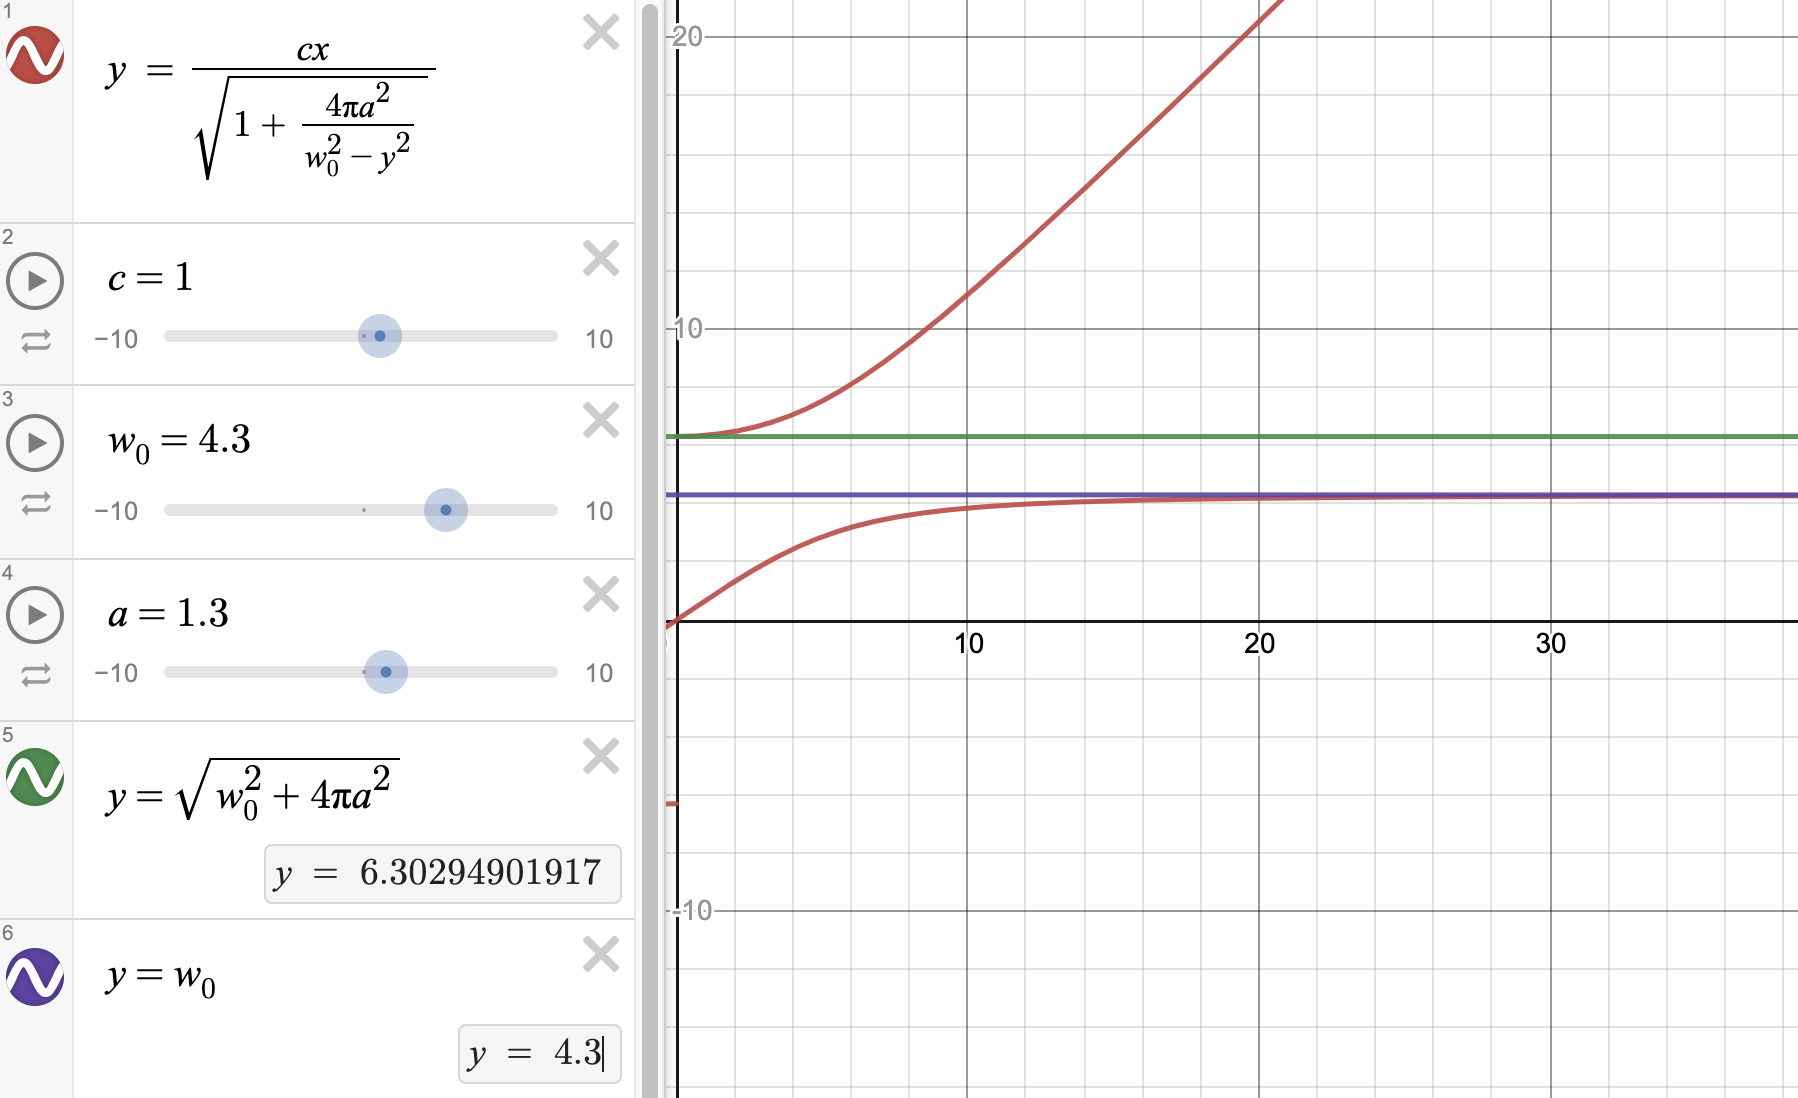
\includegraphics[width=\textwidth]{FreqWave2}
        \end{minipage}
        \hspace{0.5cm}
        \caption{Sorry this isn't bigger and for the overall quality. The y-axis shows $\omega$ and the x-axis is $k$. }
    \end{figure}
\end{frame}

In the $k \to 0$ limit, and for $\omega > \sqrt{ \omega_0^2  + 4\pi a^2 }$,  we have $\omega \to \sqrt{ \omega_0^2  + 4\pi a^2 } $. For $\omega < \omega_0$, we have $\omega \to ck / \sqrt{ \epsilon(0)} $. \\


In the $k \to \infty$ limit, and for $\omega > \sqrt{ \omega_0^2  + 4\pi a^2 }$,  we have $ \omega \to ck$. For $\omega < \omega_0$, we have $\omega \to \omega_0$. 









\end{enumerate}

\newpage

{\bf References}

\begin{enumerate}[(1)]

\item J. Schwinger et al., {\it Classical Electrodynamics}.

\item J.D. Jackson, {\it Classical Electrodynamics}.


\end{enumerate}

\begin{center}
\noindent\rule{15cm}{0.4pt} \\
\end{center}
$$\clubsuit$$
\end{document}





%+ \lambda \frac{\hbar c\alpha}{|\bm{r}_1 - \bm{r}_2|}




%\begin{equation}
%\begin{split}
%\end{split}
%\end{equation}

\begin{center}
\noindent\rule{15cm}{0.4pt} \\
\end{center}
$$\clubsuit$$
\end{document}





%+ \lambda \frac{\hbar c\alpha}{|\bm{r}_1 - \bm{r}_2|}




%\begin{equation}
%\begin{split}
%\end{split}
%\end{equation}
